
\documentclass{beamer}
\usepackage{graphicx}
\usepackage{subfigure}

\mode<presentation> {

% The Beamer class comes with a number of default slide themes
% which change the colors and layouts of slides. Below this is a list
% of all the themes, uncomment each in turn to see what they look like.

%\usetheme{default}
%\usetheme{AnnArbor}
%\usetheme{Antibes}
%\usetheme{Bergen}
%\usetheme{Berkeley}
%\usetheme{Berlin}
%\usetheme{Boadilla}
%\usetheme{CambridgeUS}
%\usetheme{Copenhagen}
%\usetheme{Darmstadt}
%\usetheme{Dresden}
%\usetheme{Frankfurt}
%\usetheme{Goettingen}
%\usetheme{Hannover}
%\usetheme{Ilmenau}
%\usetheme{JuanLesPins}
%\usetheme{Luebeck}
%\usetheme{Madrid}
%\usetheme{Malmoe}
%\usetheme{Marburg}
%\usetheme{Montpellier}
%\usetheme{PaloAlto}
\usetheme{Pittsburgh}
%\usetheme{Rochester}
%\usetheme{Singapore}
%\usetheme{Szeged}
%\usetheme{Warsaw}

% As well as themes, the Beamer class has a number of color themes
% for any slide theme. Uncomment each of these in turn to see how it
% changes the colors of your current slide theme.

%\usecolortheme{albatross}
%\usecolortheme{beaver}
%\usecolortheme{beetle}
%\usecolortheme{crane}
%\usecolortheme{dolphin}
%\usecolortheme{dove}
%\usecolortheme{fly}
%\usecolortheme{lily}
%\usecolortheme{orchid}
%\usecolortheme{rose}
%\usecolortheme{seagull}
%\usecolortheme{seahorse}
%\usecolortheme{whale}
%\usecolortheme{wolverine}
\usecolortheme{owl}

%\setbeamertemplate{footline} % To remove the footer line in all slides uncomment this line
\setbeamertemplate{footline}[page number] % To replace the footer line in all slides with a simple slide count uncomment this line

\setbeamertemplate{navigation symbols}{} % To remove the navigation symbols from the bottom of all slides uncomment this line
}

\usepackage{graphicx} % Allows including images
\usepackage{booktabs} % Allows the use of \toprule, \midrule and \bottomrule in tables
%\usepackage {tikz}
\usepackage{tkz-graph}
\GraphInit[vstyle = Shade]
\tikzset{
  LabelStyle/.style = { rectangle, rounded corners, draw,
                        minimum width = 2em, fill = yellow!50,
                        text = red, font = \bfseries },
  VertexStyle/.append style = { inner sep=5pt,
                                font = \normalsize\bfseries},
  EdgeStyle/.append style = {->, bend left} }
\usetikzlibrary {positioning}
%\usepackage {xcolor}
\definecolor {processblue}{cmyk}{0.96,0,0,0}
%----------------------------------------------------------------------------------------
%	TITLE PAGE
%----------------------------------------------------------------------------------------

\title[Short title]{How does a bike-share navigate speedy success?} % The short title appears at the bottom of every slide, the full title is only on the title page

\author{Phuc Nguyen} % Your name

\date{April 2023} % Date, can be changed to a custom date

\begin{document}

\begin{frame}
\titlepage % Print the title page as the first slide
\end{frame}

%\begin{frame}
%\frametitle{Overview} % Table of contents slide, comment this block out to remove it
%\tableofcontents % Throughout your presentation, if you choose to use \section{} and \subsection{} commands, these will automatically be printed on this slide as an overview of your presentation
%\end{frame}

%----------------------------------------------------------------------------------------
%	PRESENTATION SLIDES
%----------------------------------------------------------------------------------------

%------------------------------------------------

\begin{frame}{Problem identification}
    \begin{itemize}
        \item Cyclistic is a bike-sharing company based in Chicago.
        \item Annual members are more profitable than casual riders.
        \item How to organize a marketing campaign to convert more casual riders to members ?
    \end{itemize}
\end{frame}

\begin{frame}{Data source}
\begin{itemize}
    \item Data made publicly available by Motivate International Inc. 
    \item License found here: https://ride.divvybikes.com/data-license-agreement.
    \item No personally identifiable information.
\end{itemize}
\end{frame}

\begin{frame}{Data cleaning}
\begin{itemize}
    \item ride\_ID are mutually distinct, have same length
    \item rideable\_type has 3 values: electric bike, classic bike, docked bike.
    \item Datetimes in started\_at and ended\_at are sensible.
    \item Plotted latitudes and longitudes of stations on a map of Chicago.
    \item member\_casual has 2 values: member or casual.
\end{itemize}
\end{frame}

\begin{frame}{Members vs casual}
\begin{figure}
\includegraphics[width=0.75\textwidth]{Average Trip Duration}\\
Casual riders ride longer (tourism vs commuting).
\end{figure}
\end{frame}

\begin{frame}{Cold season vs warm season}
\begin{figure}
\begin{subfigure}{}
  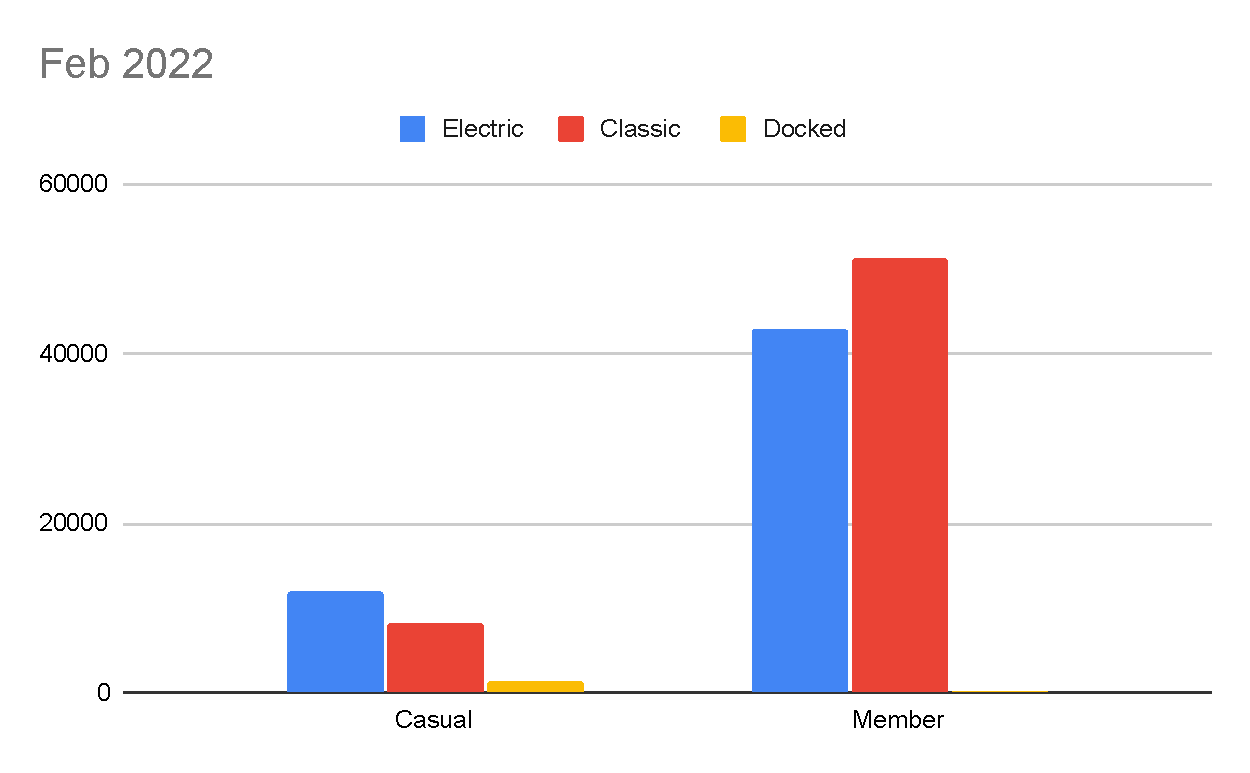
\includegraphics[width=.5\textwidth]{Feb2022RideBreakdown}
\end{subfigure}%
\begin{subfigure}{}
  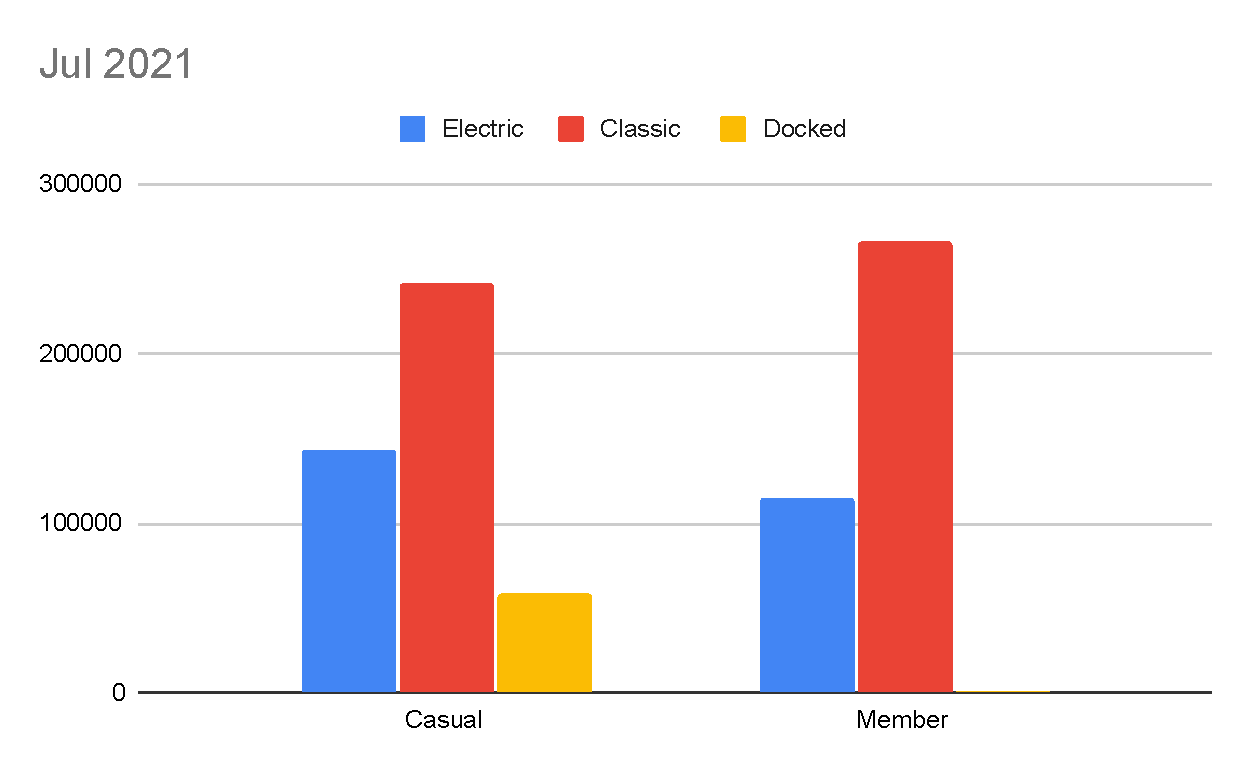
\includegraphics[width=.5\textwidth]{Jul2021RideBreakdown}
\end{subfigure}
\end{figure}
More rides in the summer than winter. (tourism picks up in the summer.)
\end{frame}

\begin{frame}{Weekday vs weekend}
\begin{figure}
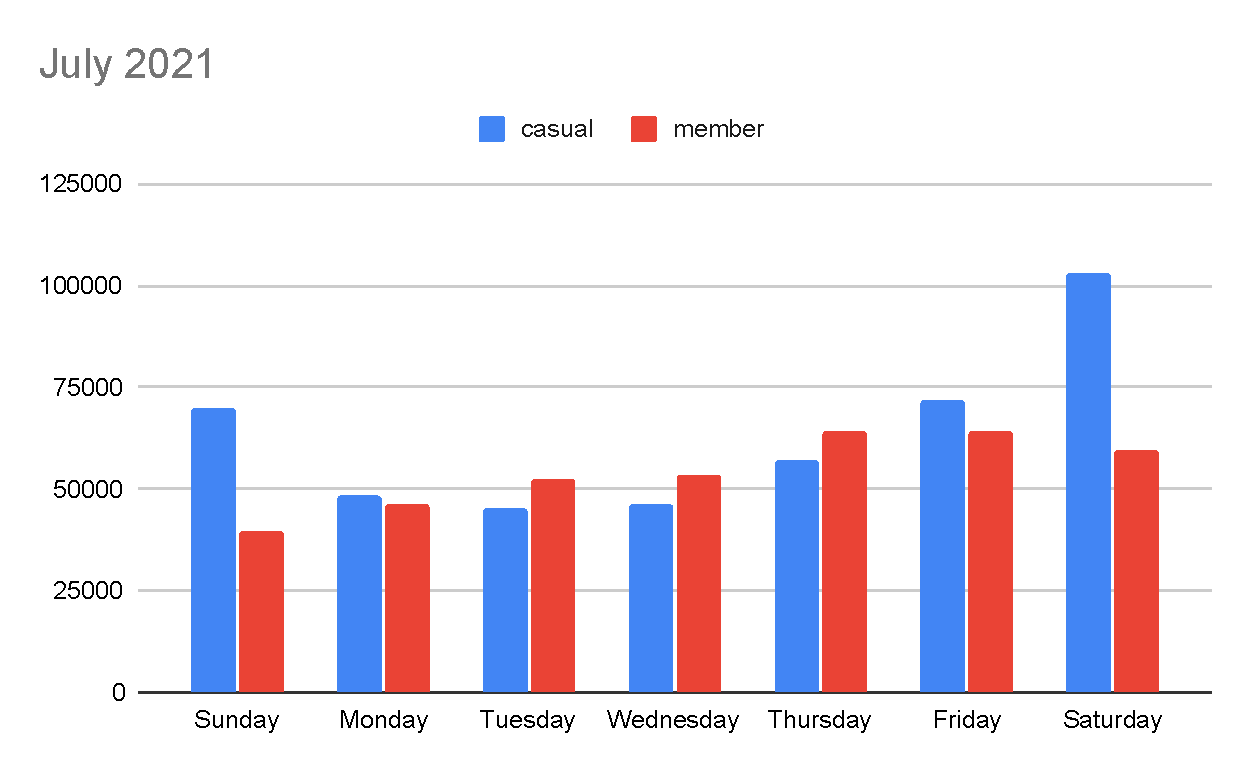
\includegraphics[width=0.75\textwidth]{July_2021}\\
For casual riders, ridership peaks at weekend. (again, because it's leisure and sightseeing)
\end{figure}
\end{frame}

\begin{frame}{Breakdown by hour of the day}
\begin{figure}
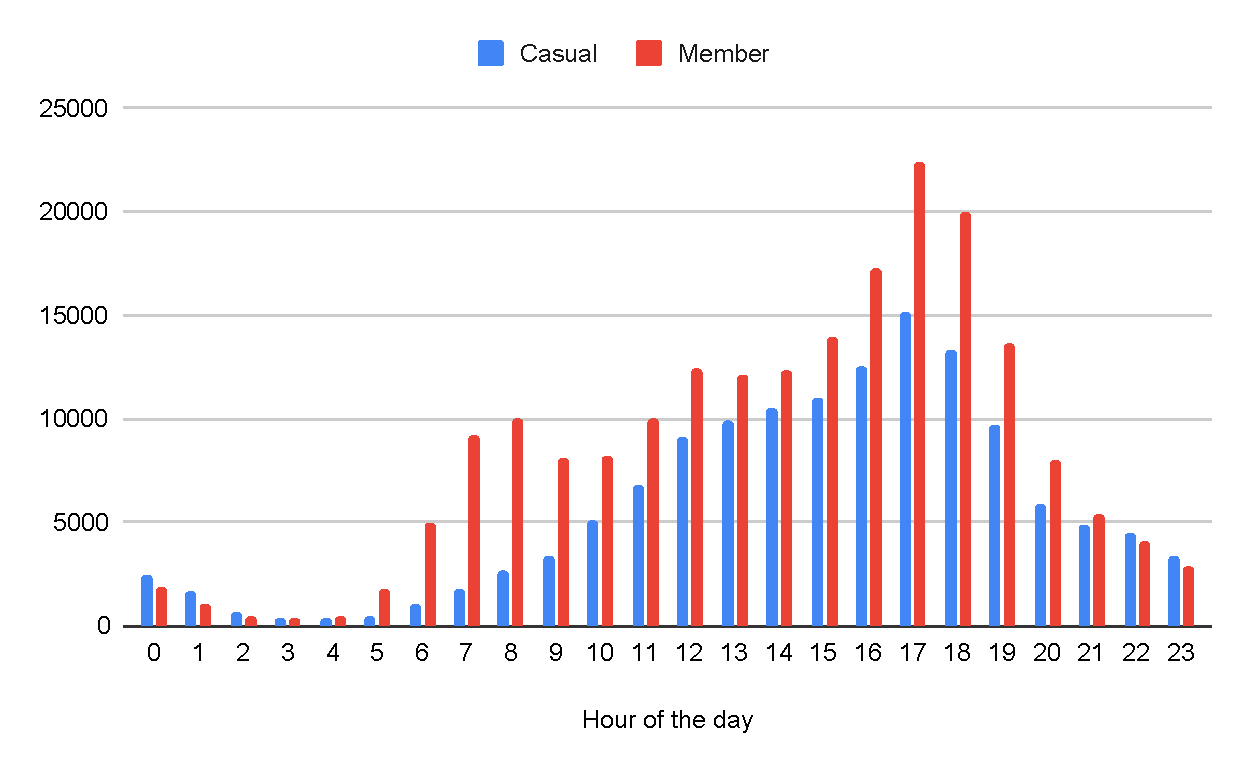
\includegraphics[width=0.75\textwidth]{BreakdownByHour}\\
For members, ridership peaks at rush hour, both morning and evening. (because they commute)
\end{figure}
\end{frame}

\begin{frame}{Geographically}
\begin{figure}
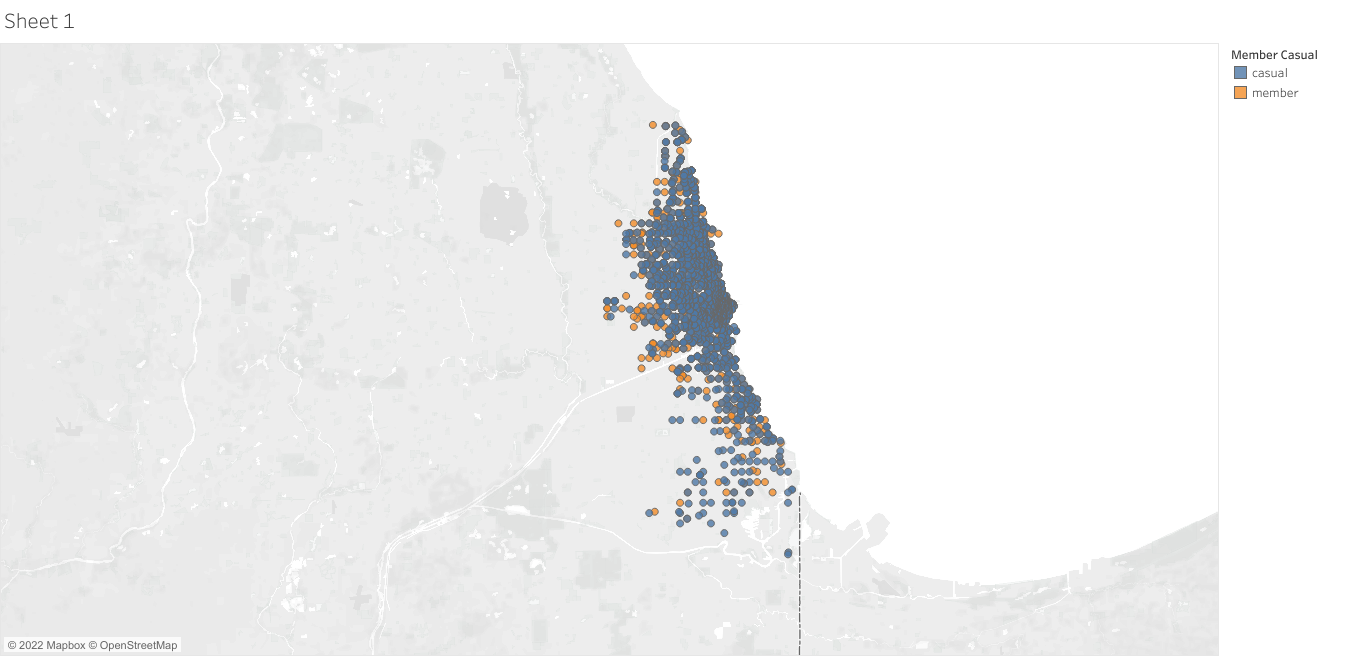
\includegraphics[width=0.8\textwidth]{Sheet_1}\\
Geographically, both casual riders and members seem evenly spread out across Chicago.
\end{figure}
\end{frame}

\begin{frame}{Recommendations}
\begin{itemize}
    \item Offer discounts for signing up for memberships for riders who ride for longer periods (because they tend to be casual riders);
    \item Organize marketing campaigns during the warmer months (when there are more casual riders);
    \item or near famous tourist attractions in Chicago (because the casual riders ride for tourism).
\end{itemize}
\end{frame}

\end{document}